\newpage
\section{Galaxy Integration}
A spectrum represents the intensity of light being emitted over a range of energies (i.e. frequencies). One can analyze the light from stars and galaxies using spectral gratings to study their features. A galaxy spectrum, in particular, will tell you about the types of stars the galaxy contains, the relative abundances of each type of star, and many more.

Galaxy spectra are typically characterized by a strong continuum component caused by the combination of a range of blackbody emitters spanning a range in temperature. 
However, stars are also surrounded by
thin gas, which either emits or absorbs light at only a specific set of frequencies,
causing spectral lines. Every chemical element produces a specific set of lines at fixed frequencies, so by identifying the lines, we can tell what types of atoms and molecules a star is made of. If the gas is cool, then it will absorb light at these wavelengths, and if the gas is hot, then it will emit light at these
wavelengths. 
% For galaxies, on the other hand, we expect mostly emission spectra.

The strength of each emission line (in W/m$^2$) is defined as the relative intensity
of each peak across the associated frequencies.
The problem at hand is to develop a process for analyzing galaxy spectra so as
to determine the strength of each of the emission lines.

\subsection{Algorithm}
The algorithm to analyse galaxy spectrum data to find the line strengths can be divided into two parts -- (i) cleaning up raw data along with detection of emission lines and (ii) finding the relative strength of each emission line. 

\subsubsection{Data Cleanup \& Finding Emission Lines}
To find emission lines, we will follow the following procedure. For demonstration, we will be working with spectra of NGC 1275.\\

\noindent \textbf{Step 1: Continuum Subtraction}\\
\noindent The continuum represents the sum of the blackbody radiation emitted by objects in the galaxy. To integrate the emission lines, we first need spectrum sans the continuum. The standard approach to this is to approximate a spectrum to a blackbody function using Chebyshev polynomials. However, since we are only dealing with a small section of the blackbody curve, we can roughly approximate it with a straight line. But depending on the spectrum, we can use different kinds of curve fittings.

\begin{lstlisting}[language=Python, caption=Implementation of Linear Regression for straight line fitting compared with the standard specutils library generic continuum fit]
def linregress(x, y):
    n = len(x)
    Sxx = x@x
    Sxy = x@y
    Sy = np.sum(y)
    Sx = np.sum(x)
    delta = n*Sxx - (Sx)**2
    slope = (n*Sxy - Sx*Sy) / delta
    intercept = (Sxx*Sy - Sx*Sxy) / delta
    return slope, intercept

plt.plot(frequency, intensity, 'k', label='Observed spectrum', alpha=0.5)  

# using specutils package
spectrum = Spectrum1D(flux=intensity*u.Jy, spectral_axis=lambda_*u.angstrom)
g1_fit = fit_generic_continuum(spectrum)
y_continuum_2 = g1_fit(lambda_*u.angstrom)
flux = intensity/y_continuum_2
plt.plot(frequency, y_continuum_2, 'b--', label='Continuum fit using\nspecutils package')

# using least square fitting
slope, intercept = linregress(frequency, intensity)
y_continuum_1 = slope*frequency+intercept
plt.plot(frequency, y_continuum_1, 'r:', label='Continuum using Least-Square\nStraight line fit')

flux = intensity/y_continuum_1 # continuum subtracted intensity
\end{lstlisting}

Fig. \ref{continuum} shows the straight line fit along with the Chebyshev polynomial fit (using \verb|astropy|'s \verb|specutils| package) on top of the observed spectrum.

\begin{figure}[H]
    \centering
    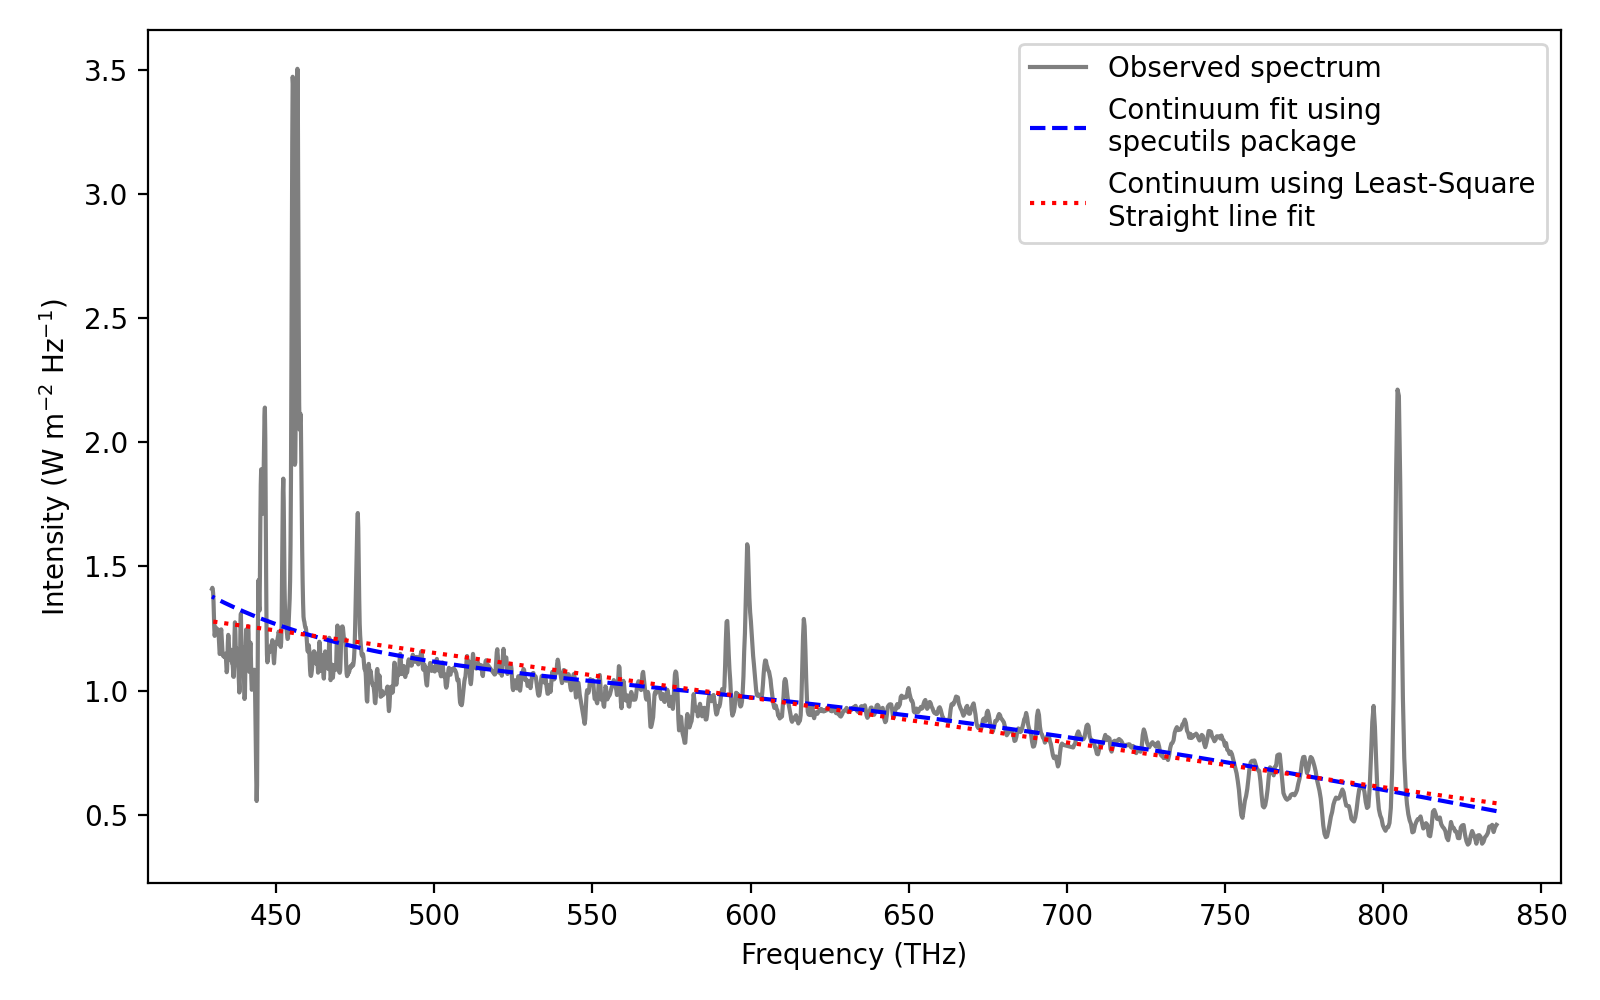
\includegraphics[width=0.7\linewidth]{Figures/3/continuum.png}
    \caption{Continuum fit of the galaxy spectrum}
    \label{continuum}
\end{figure}

The continuum subtracted spectrum is obtained by dividing the original spectrum by the fitted continuum. This approach preserves the features of the spectrum better than simple subtraction of the continuum from the original.

\begin{figure}[H]
    \centering
    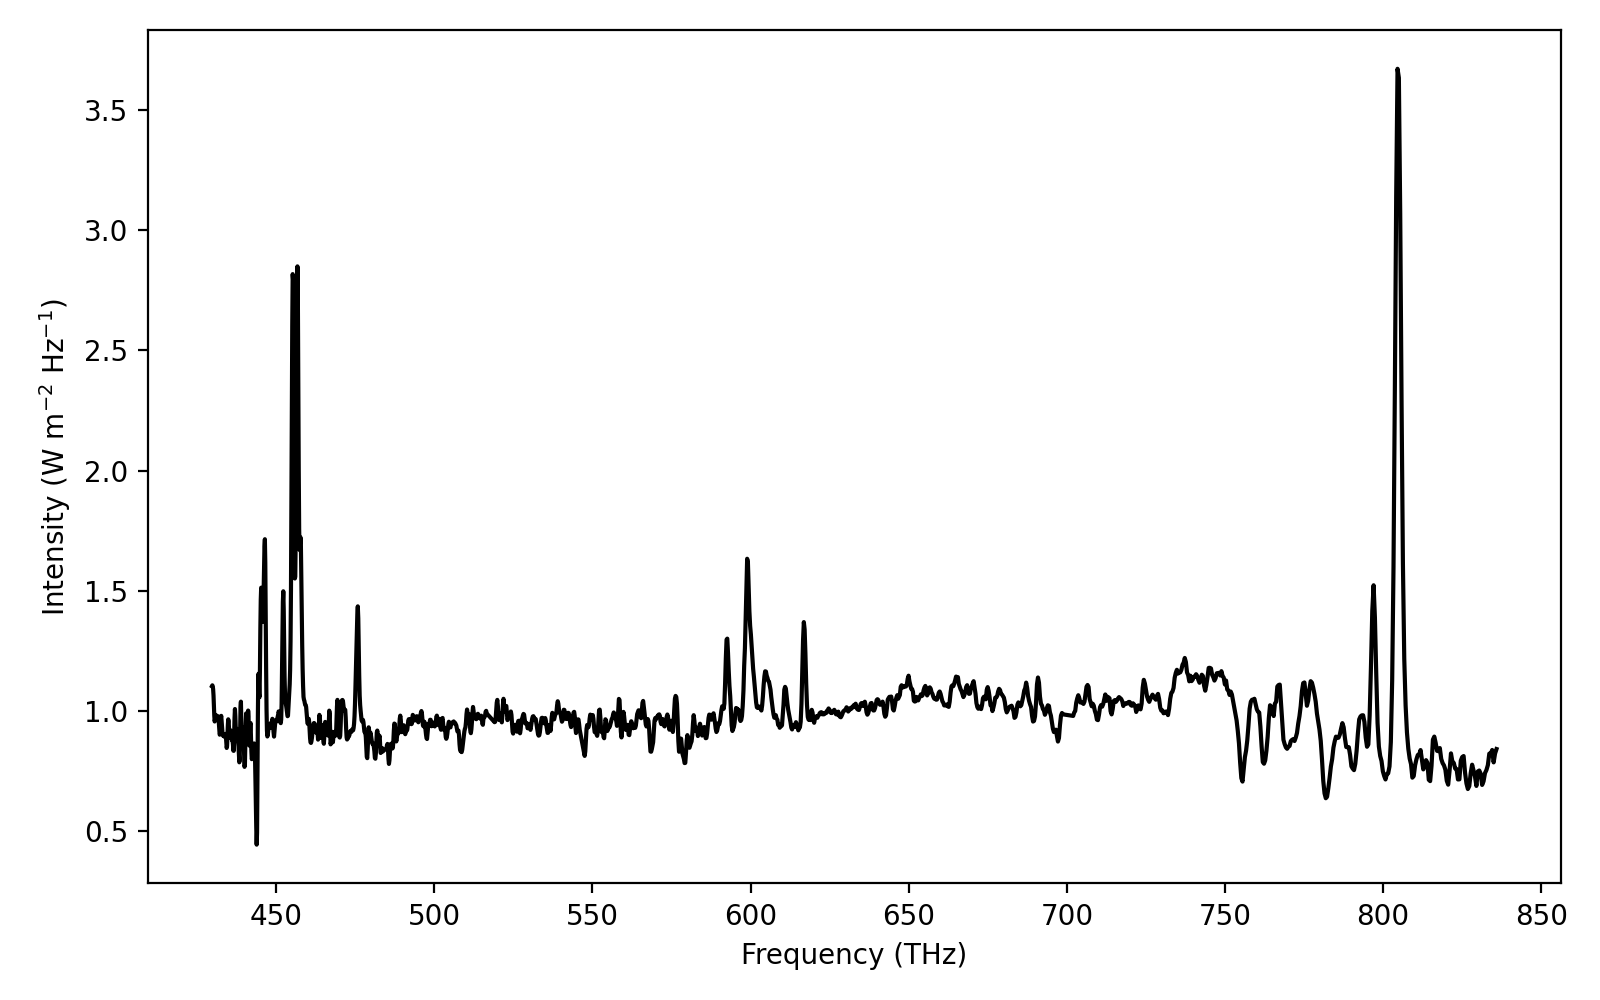
\includegraphics[width=0.7\linewidth]{Figures/3/continuum_sub.png}
    \caption{Continuum subtracted galaxy spectrum}
\end{figure}

\noindent \textbf{Step 2: Smoothening the Spectrum}\\
\noindent The background noise can be greatly reduced by applying a median filter over the spectrum. This makes line finding easier and less prone to error due to random spikes in
the spectrum. The median filter acts by acting on each point,

\begin{align}
    f[i] = \text{median}(f[i-1], f[i], f[i+1])
\end{align}

We can also increase the kernel of this median filter by including more neighbouring points in the above equation. However, that has the disadvantage of possibly distorting emission line strengths.

\begin{lstlisting}[language=Python, caption=Implementation of median filter with kernel k = 3 (i.e. median along two neighbouring points)]
def medfiltt(x, k=3):
    n = len(x)
    xs = np.zeros(n)
    for i in range(n):
        a = i-k if i >= k else 0
        b = i+k if i <= n-k else -1 
        xs[i] = np.median(x[a:b])
    return xs

flux_smooth = medfiltt(flux)
\end{lstlisting}

\noindent \textbf{Step 3: Finding emission lines}\\
\noindent The simplest method to find emission lines is to calculate the derivative at every point and classify the ones that are above a certain threshold value. However, due to the high amount of noise in the spectrum, we need to include as many neighbouring points as possible in calculating the first derivative.

Eqn. \ref{firstderivative} is the first-order approximation of the first derivative using the central difference method, with an order $O(h^2)$ error. Using Richardson Extrapolation, one can increase the accuracy of this formula. Here, we have performed Richardson Extrapolation thrice to arrive at the 4th-order approximation of the first derivative.

Richardson extrapolation is given by,

\begin{align}
    G = \frac{2^p g(h/2) - g(h)}{2^p - 1} + O(h^{p+q})
\end{align}

where $G$ is the quantity we are after and $g(h)$ is the approximate quantity using a step size $h$. $p$ and $q$ represent the order of the leading error term and the increment in the order for the error terms after that, respectively. Using $p=2$ and $q=2$ in Eqn. \ref{firstderivative},

\begin{align}
    f'(x) \approx \frac{8(f(x+h) - f(x-h)) - f(x+2h) + f(x-2h)}{12h} + O(h^4) 
\end{align}

Again, if we perform the same procedure two more times,

\begin{align}
    f'(x) &\approx \frac{15(f(x+h) - f(x-h)) - 9((f(x+2h) + f(x-2h)) + ((f(x+3h) + f(x-3h))}{12h} + O(h^6)\\
    f'(x) &\approx \frac{4}{5}(f(x+h) - f(x-h)) - \frac{1}{5}(f(x+2h) - f(x-2h)) + \frac{4}{105}(f(x+3h) - f(x-3h)) \nonumber\\
    &- \frac{1}{280}(f(x+4h) - f(x-4h)) + O(h^8)
\end{align}

\begin{lstlisting}[language=Python, caption=Implementation of the 4th order approximation of the first derivative]
def dydx(y):
    dy = np.zeros(len(y))    
    for i in range(4, len(y)-4):
        dy[i] = (-y[i+4] + (4*280/105)*y[i+3] - 56*y[i+2] + 224*y[i+1] - 224*y[i-1] + 56*y[i-2] - (4*280/105)*y[i-3] + y[i+4])/280
            
    return dy
\end{lstlisting}

The inclusion of more neighbouring points in the derivative effectively minimises the effect of random spikes of noise in the data.

Practically, the peaks were found by setting a threshold value for the first derivative along with a threshold value for the continuum subtracted spectrum. In order to avoid really closely spaced peaks, we have also implemented a simple for loop to remove any peaks within $\sim$ 10 THz of each other.

\begin{lstlisting}[language=Python, caption=Finding the peaks using a threshold value set manually]
threshold = 0.080
flux_smooth = medfiltt(flux, 1)
dy4 = dydx(flux_smooth, 4)
line_fs = frequency[np.where((dy4>threshold) & (flux_smooth>1.3))]
realines = []
i = 0
while i < len(line_fs):
    realines.append(line_fs[i])
    for j in range(i+1, len(line_fs)):
        if abs(line_fs[i] - line_fs[j]) <= 10:
            i += 1
    i += 1
\end{lstlisting}

\begin{figure}[H]
    \centering
    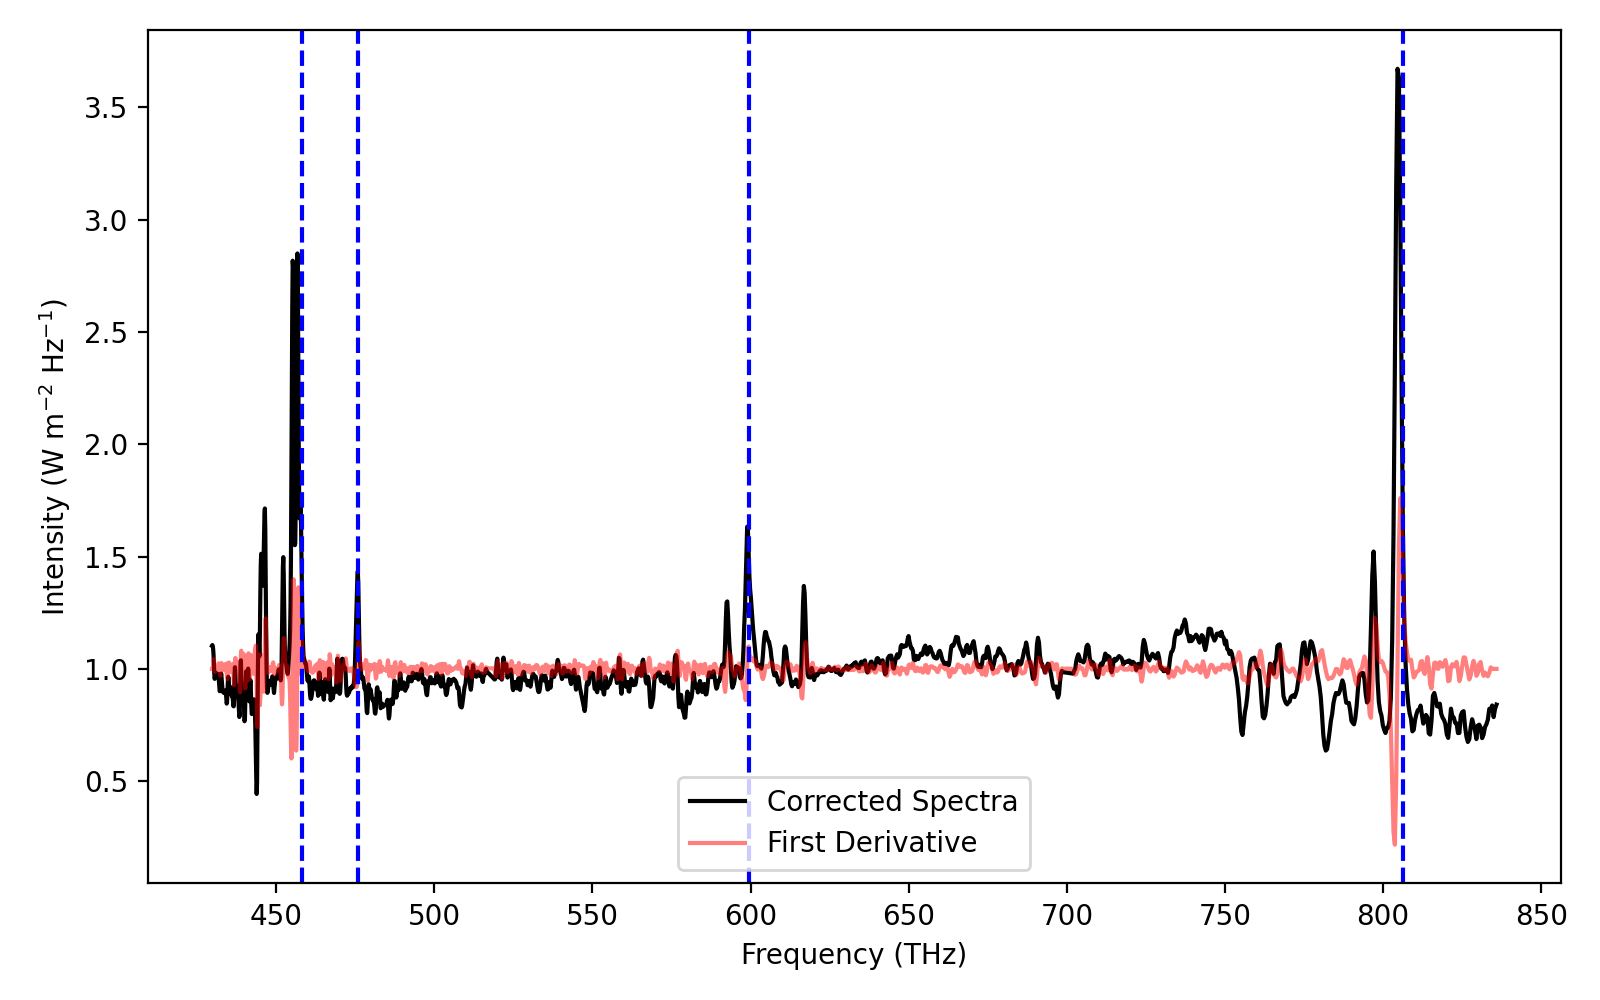
\includegraphics[width=0.7\linewidth]{Figures/3/peaks.png}
    \caption{Major emission peaks detected for our observed spectrum. The red line indicates the first derivative of the continuum subtracted spectrum.}
\end{figure}

\subsubsection{Finding Line Strengths}

Now, let us examine each peak closely.

\begin{figure}[H]
    \centering
    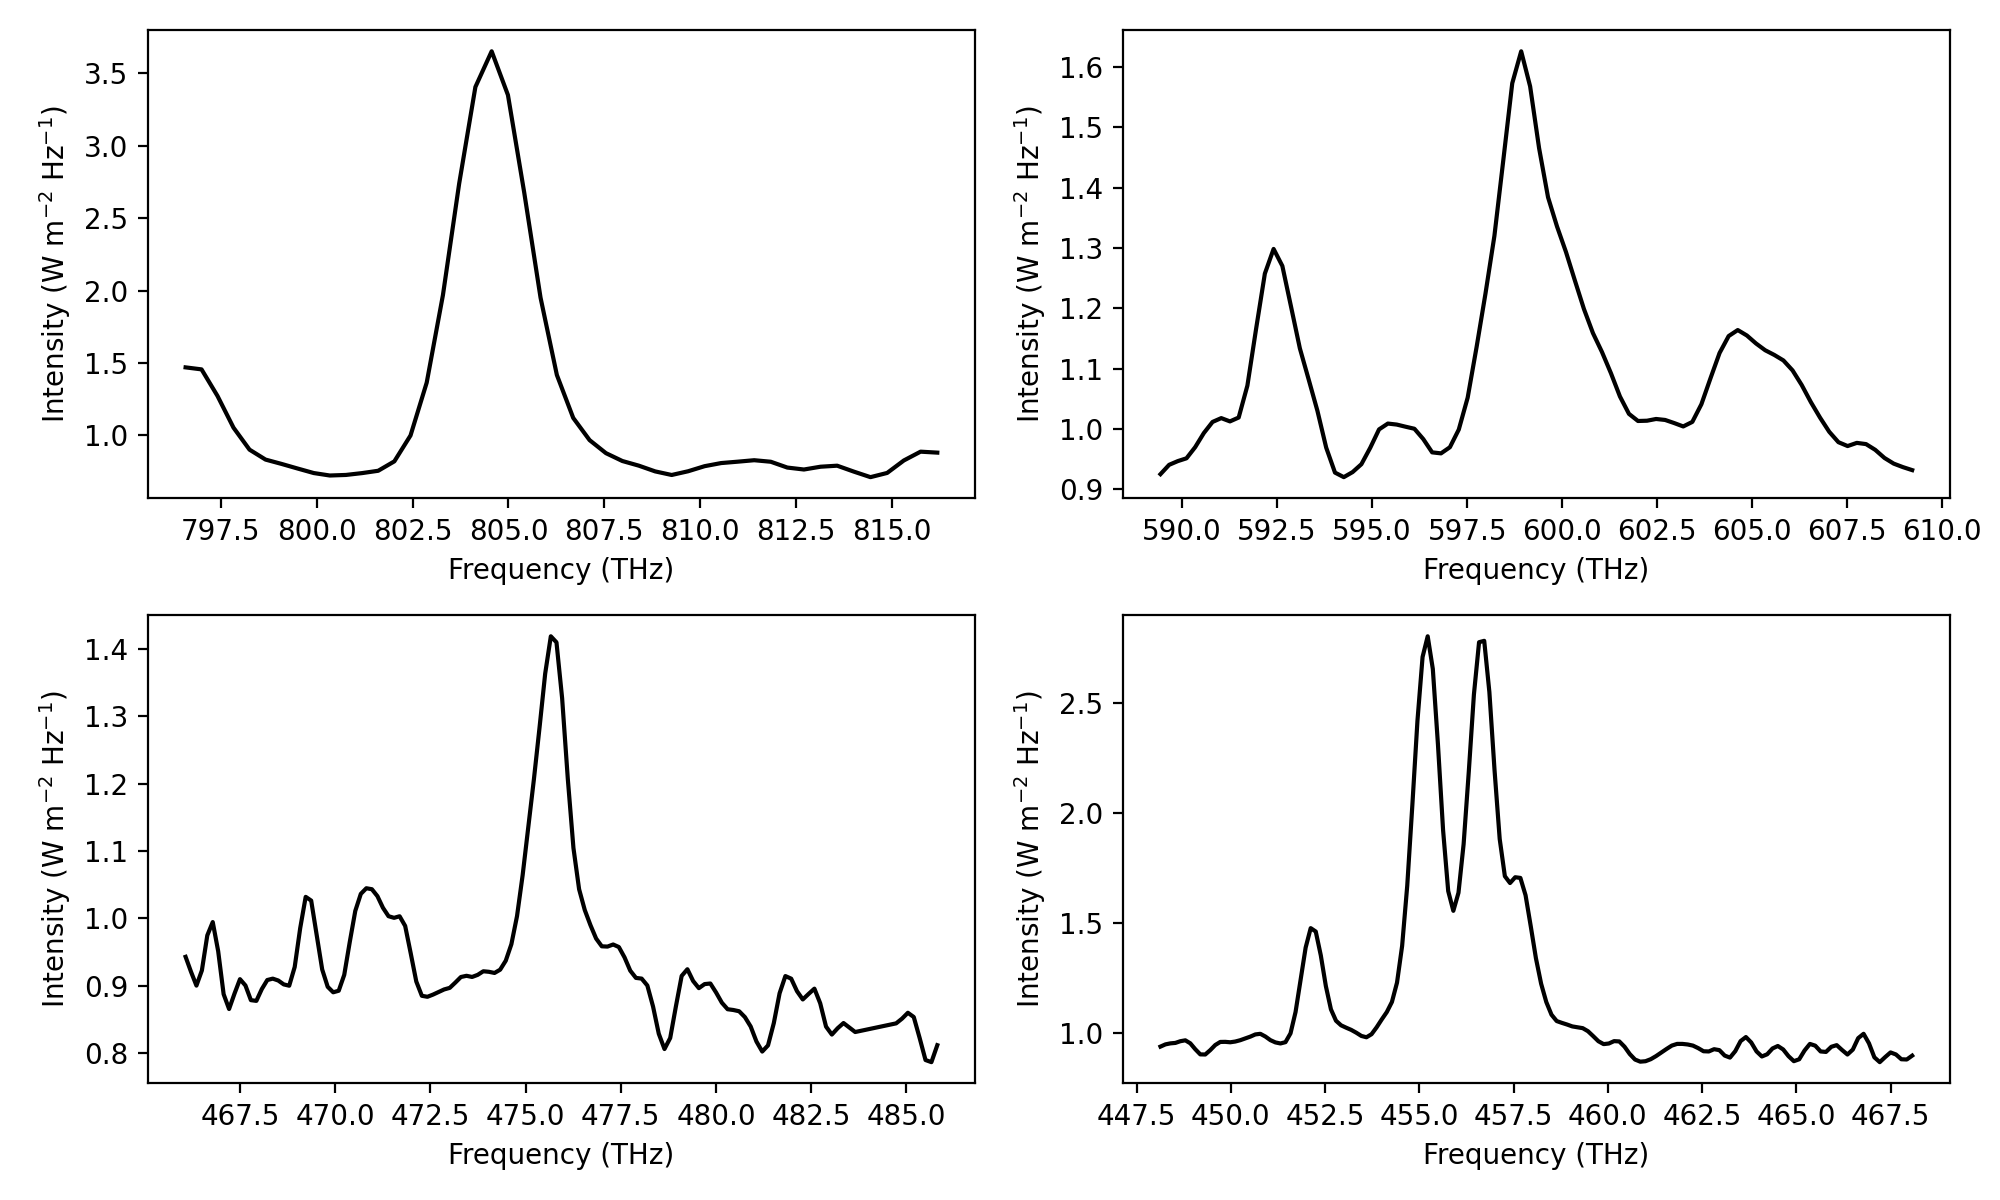
\includegraphics[width=0.7\linewidth]{Figures/3/peaks_zoom.png}
    \caption{Zoomed in version of the detected peaks}
\end{figure}

The strength of each emission line is given by integrating its intensity with respect to frequency (in W/m$^2$).

\begin{align}
    \text{Line Strength} = \int_{\nu_0}^{\nu_1} I(\nu) d\nu
\end{align}

However, given the noisy nature of our spectrum, numerical integration has a high degree of error associated with it. Not to mention that one has to manually figure out the integration limits in the above equation for every peak.

A more precise way to find the line strength is by considering each emission peak as a Gaussian distribution. Now, by fitting a Gaussian function on each peak window, we can determine the line strength as the area under a Gaussian distribution, given by

\begin{align}
    \text{for any } g(\nu) = Ae^{-\frac{(\nu-\nu_0)^2}{2\sigma^2}},\,\,\int_{-\infty}^{\infty} g(\nu) d\nu = A\sigma\sqrt{2\pi}
\end{align}

By using \verb|scipy.curve_fit()|, we have fit Gaussian functions over every curve using our initial estimate.

\begin{lstlisting}[language=Python, caption=Finding the peaks using a threshold value set manually]
from scipy.optimize import curve_fit 

def gaussian(x, amplitude=1, mean=0, stddev=1): 
    y = amplitude*np.exp(-((x-mean)**2)/(2*stddev)) 
    return y 
    
for line in realines:
    window = np.where((frequency > line-10) & (frequency < line+10))
    xs = frequency[window]
    ys = flux_smooth[window] - 1
    
    plt.plot(xs, ys, 'k', alpha=1, label='Corrected Spectra')
    
    params, cov = curve_fit(gaussian, xs, ys, p0=[np.max(ys), line, 5])
    fit_x = np.linspace(xs[-1], xs[0], 200)
    fit_y = gaussian(fit_x, params[0], params[1], params[2]) 
    
    strength = params[0]*np.sqrt(params[2]*2*np.pi)
    strength_err = strength*np.sqrt(cov[0][0] + cov[2][2]/4)
    
    plt.plot(fit_x, fit_y, 'b-', label=f'Best fit Gaussian', alpha=0.5)
    plt.title(f'f = {params[1]:.2f} THz, Line Strength = ({strength:.3f} '+ r"$\pm$"+ f' {strength_err:.3f}) W/m'+r"$^{2}$", fontsize=10)
    final_lines[params[1]] = (strength, strength_err)
    
    plt.ylabel('Intensity (W m$^{-2}$ Hz$^{-1}$)')
    plt.xlabel('Frequency (THz)')
\end{lstlisting}

The error in the estimation of $A$ and $\sigma$ from the covariance matrix is used to find the error in the line strength given by,

\begin{figure}[H]
    \centering
    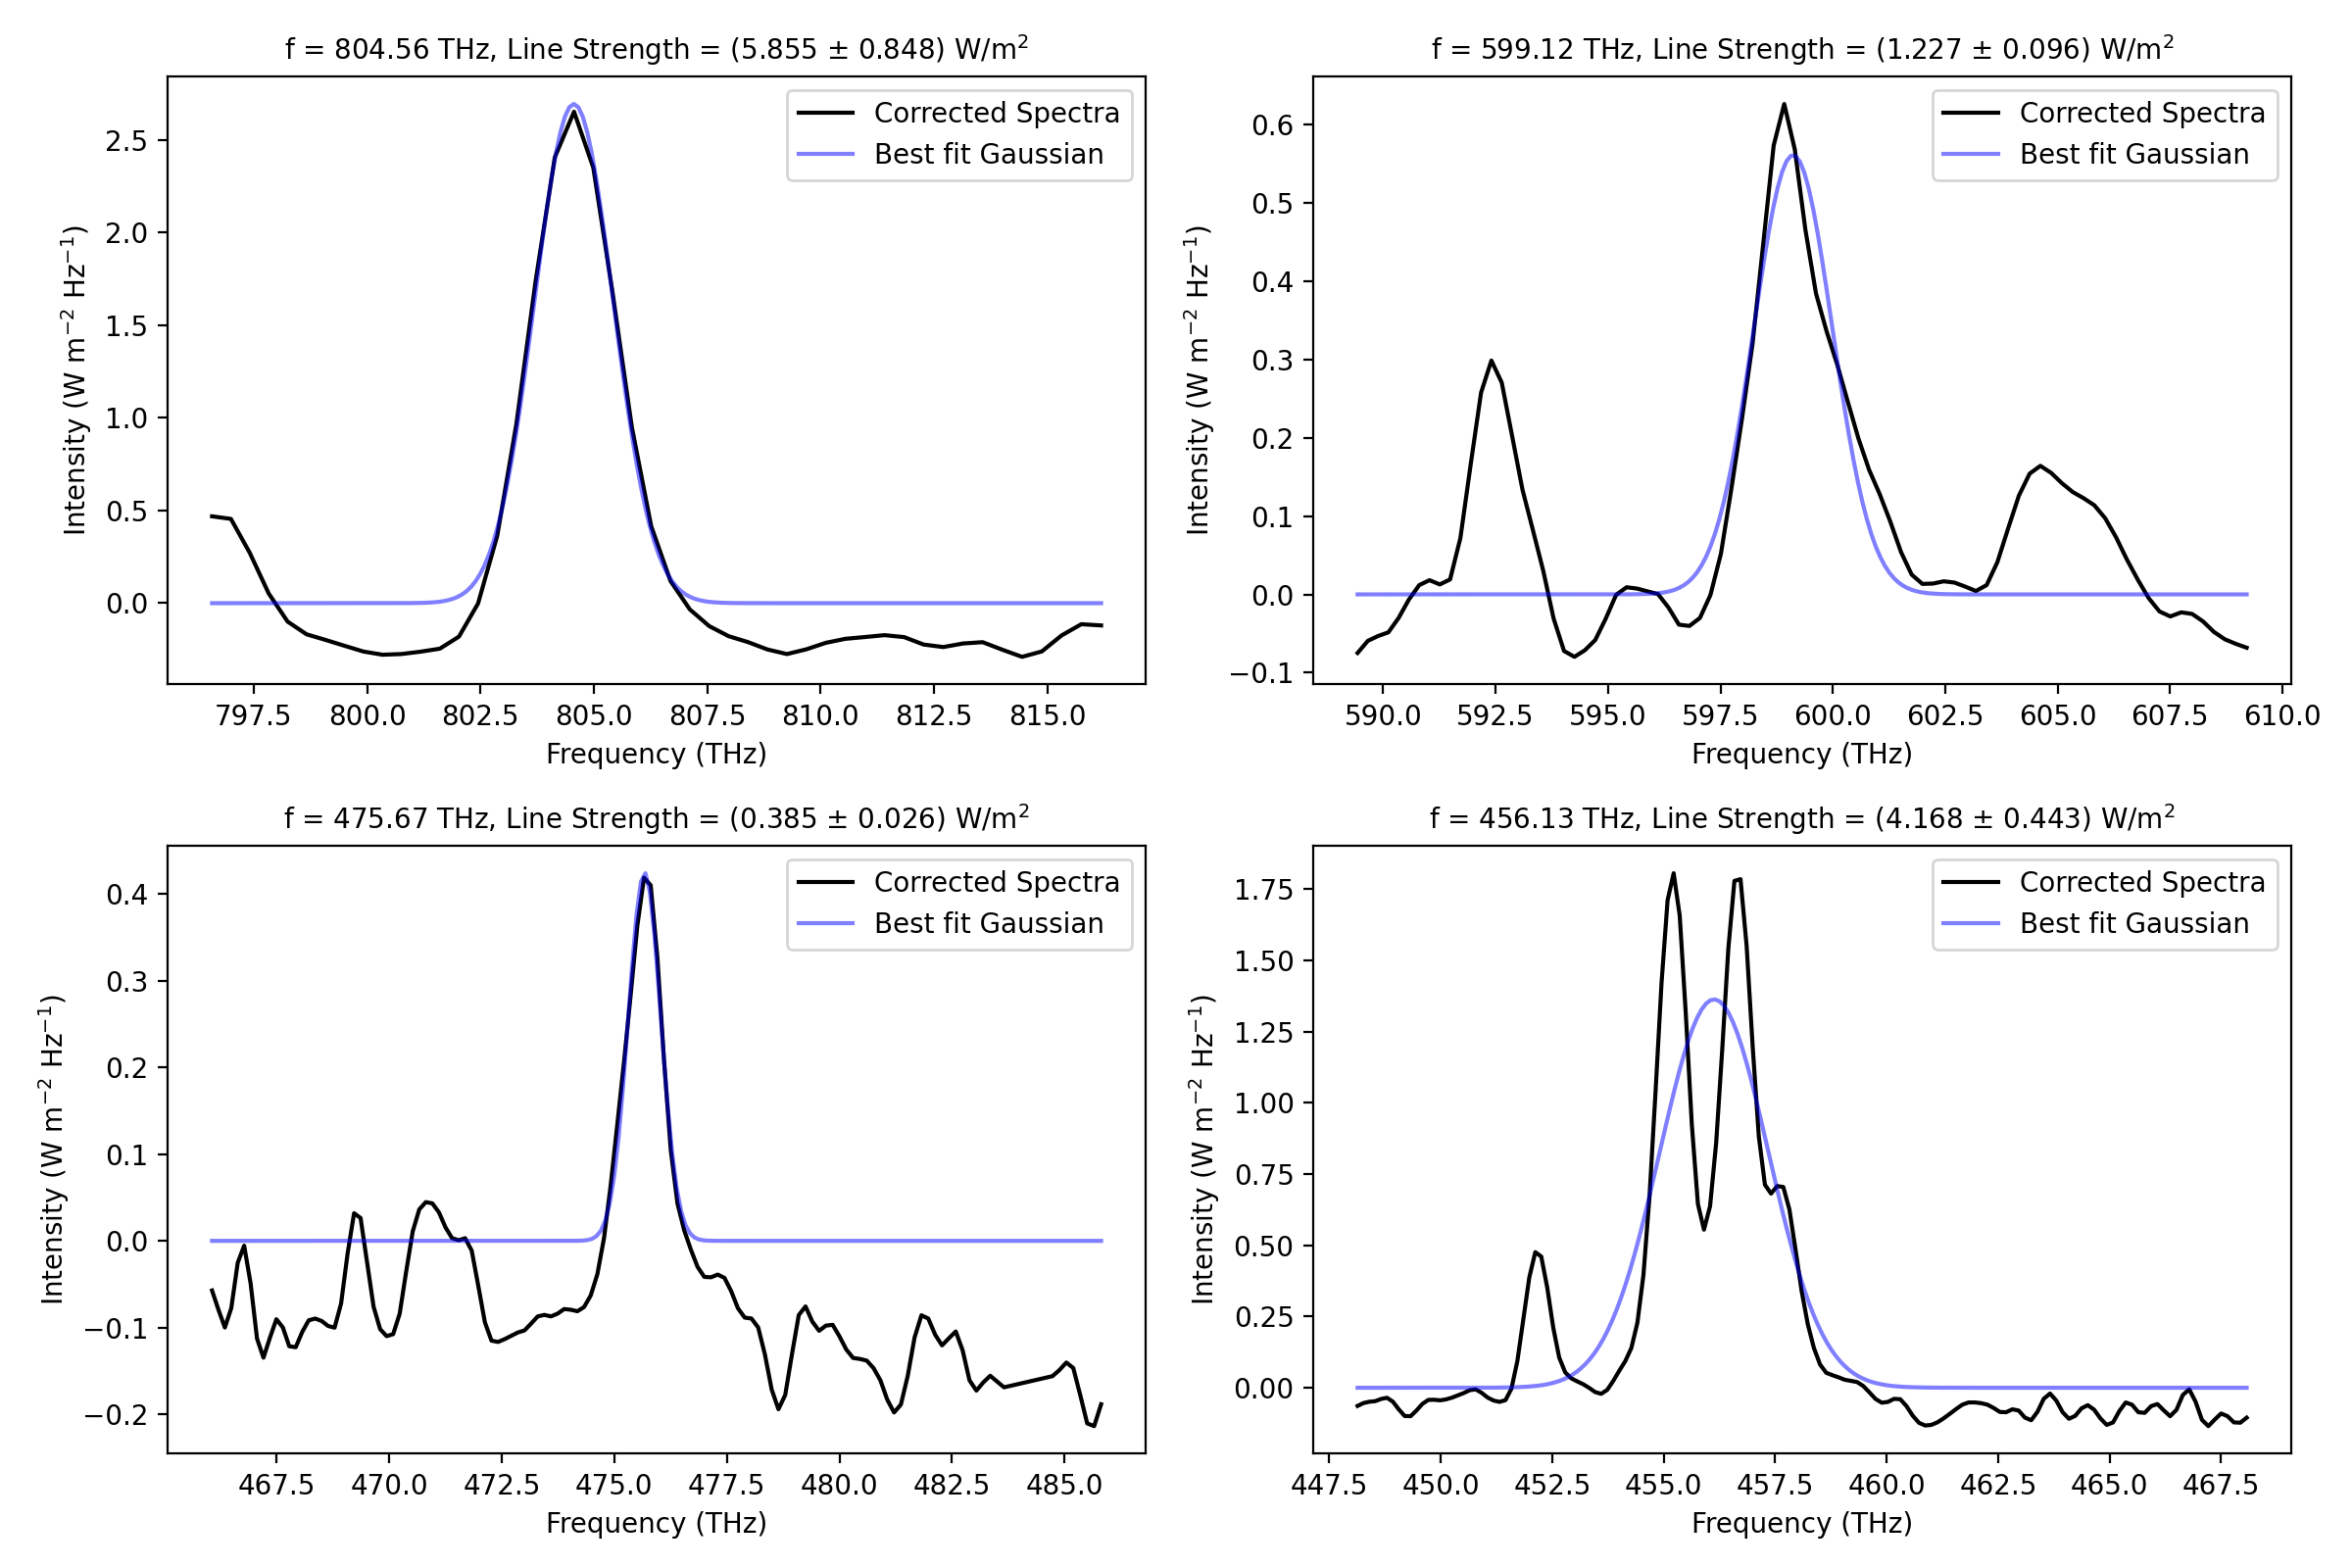
\includegraphics[width=0.9\linewidth]{Figures/3/peaks_zoom_fit.png}
    \caption{Gaussian function fitted on each emission line}
\end{figure}

The results are shown below.
\begin{align}
    \frac{\Delta \text{Line Strength}}{\text{Line Strength}} = \sqrt{\left(\frac{\Delta \sigma}{\sigma}\right)^2 + \left(\frac{\Delta A}{A}\right)^2}
\end{align}

As we can see here, the fourth panel consists of a double peak which cannot be estimated by a single Gaussian function. In such cases, we can manually change the estimation window by cutting off one of the peaks to estimate the other.

\begin{lstlisting}[language=Python, caption=Dealing with double peaks]
line1 = 455
line2 = 457

window = np.where((frequency > line-10) & (frequency < line+10))
xs = frequency[window]
ys = flux_smooth[window] - 1
plt.plot(xs, ys, 'k', alpha=1, label='Corrected Spectra')

# define the first window by cutting of the second peak
win1 = np.where(xs < line1+0.8)
params1, cov1 = curve_fit(gaussian, xs[win1], ys[win1], p0=[1.75, line1, 0.1])
win2 = np.where((xs > line2-1) & (xs < line2+0.4))
params2, cov2 = curve_fit(gaussian, xs[win2], ys[win2], p0=[2, line2, 0.5])

# define the second window by cutting of the first peak
fit_x = np.linspace(xs[-1], xs[0], 200)
fit_y1 = gaussian(fit_x, params1[0], params1[1], params1[2]) 
fit_y2 = gaussian(fit_x, params2[0], params2[1], params2[2]) 

# final curve fit is the addition of the two emission lines
plt.plot(fit_x, fit_y1+fit_y2, 'b-', label='Best fit Gaussian', alpha=0.5) 
print('Area under fit1:', params1[0]*np.sqrt(params1[2]*2*np.pi))
print('Area under fit2:', params2[0]*np.sqrt(params2[2]*2*np.pi))
strength1 = params1[0]*np.sqrt(params1[2]*2*np.pi)
strength2 = params1[0]*np.sqrt(params2[2]*2*np.pi)
strength1_err = strength1*np.sqrt(cov1[0][0] + cov1[2][2]/4)
strength2_err = strength2*np.sqrt(cov2[0][0] + cov2[2][2]/4)

final_lines[params1[1]] = (strength1, strength1_err)
final_lines[params2[1]] = (strength2, strength2_err)
\end{lstlisting}

\begin{figure}[H]
    \centering
    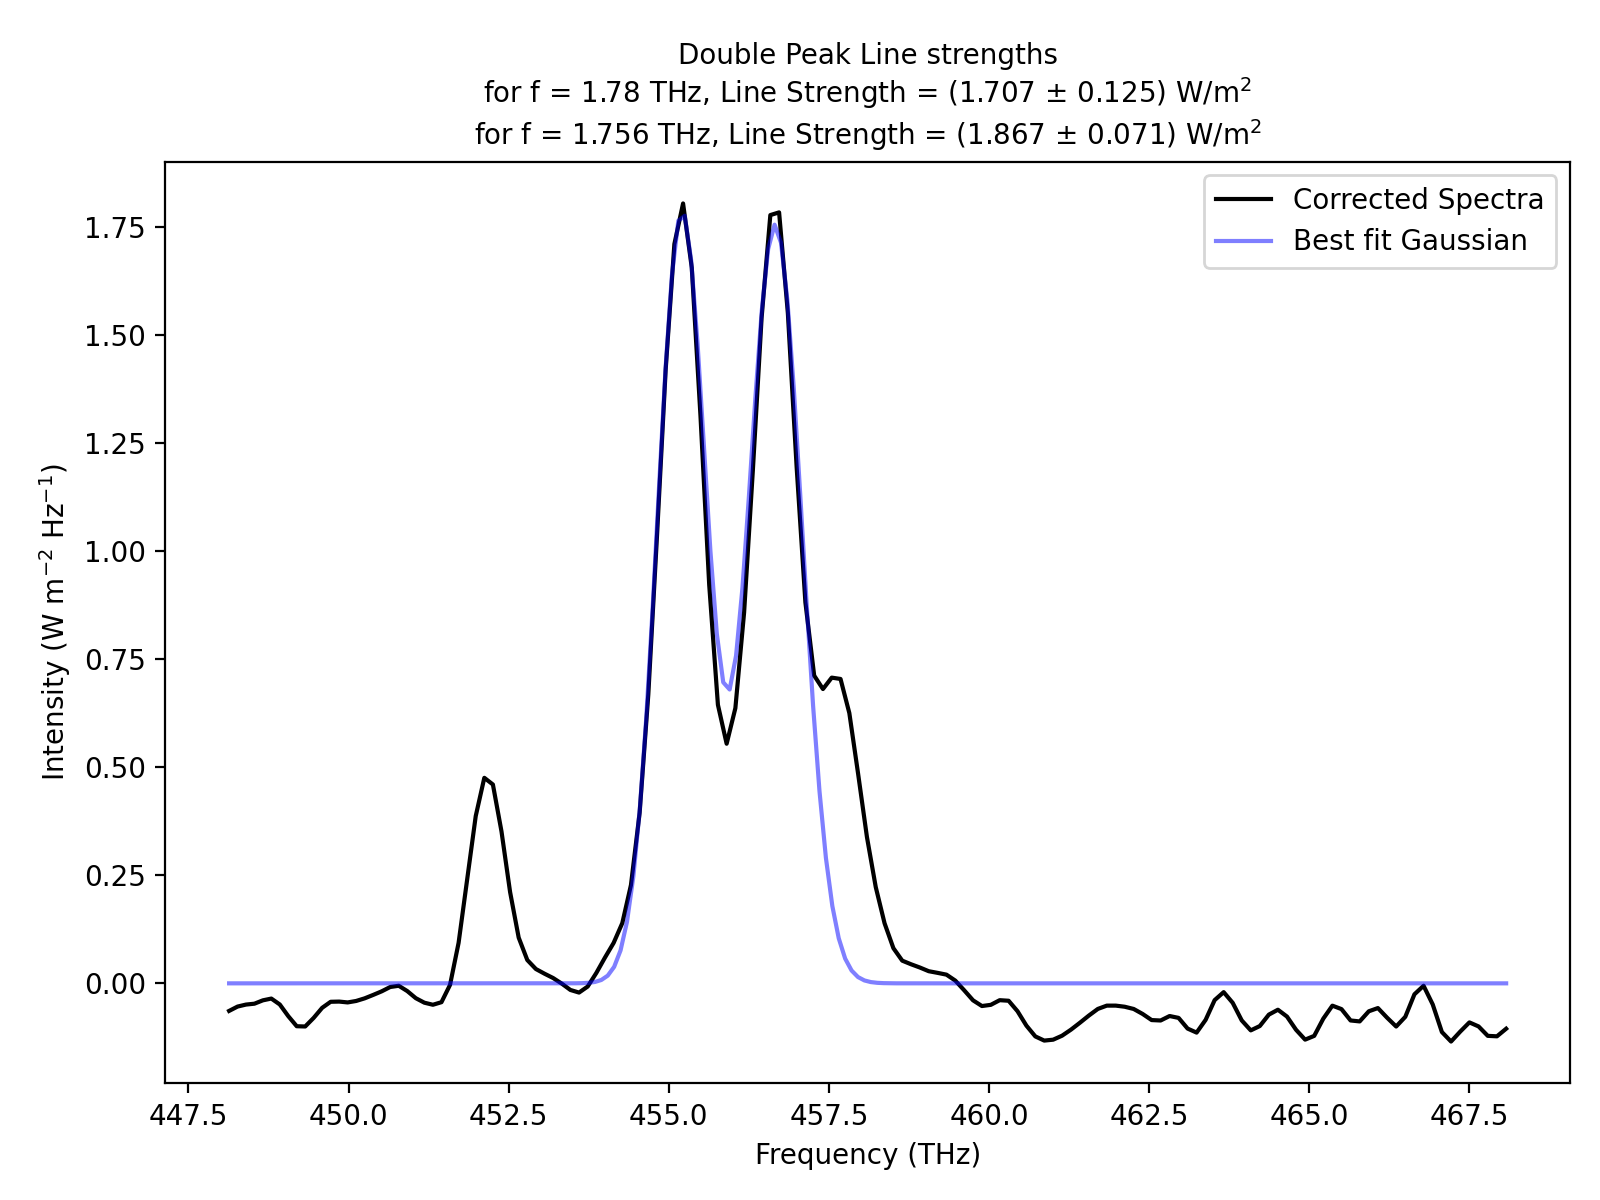
\includegraphics[width=0.6\linewidth]{Figures/3/double_peak.png}
    \caption{The double peak fitting}
\end{figure}

\subsubsection{Chemical Correspondence of Emission Lines}

Now that we have all the emission peaks along with their respective line strengths (and their error bars), all we have to do is to match them against the literature data to find the corresponding ion/molecule causing the emission. Here, we have used the Galaxy Emission Line database developed by Drew Chojnowski\footnote{\href{http://astronomy.nmsu.edu/drewski/tableofemissionlines.html}{Source.}}.

\begin{lstlisting}[language=Python, caption=Finding the closest possible emission line to match with from the database]
import pandas as pd

data = pd.read_csv('galaxy_emission_lines.csv')
print('Emission Lines Found:\n')

for line, strength in final_lines.items():
    line_w = f2w(line)
    ion = data.iloc[(data['lambda']-line_w).abs().argsort()[0]]['Ion']
    print(f'f = {line:.2f} THz ({line_w:.1f} AA), possibly due to {ion}\n  Line Strength = ({strength[0]:.3f} \pm {strength_err:.3f}) W/m^2')
\end{lstlisting}

\subsection{Results}

The results are summarised in table \ref{galaxy_summary} and Fig. \ref{galaxy_summary_pic}

\begin{table}[ht]
\rowcolors{2}{Tue-red!10}{white}
\centering
\begin{tabular}[t]{cccc}
\toprule
\color{Tue-red}\textbf{Emission frequency (THz)}&\color{Tue-red}\textbf{Wavelength (nm)}&\color{Tue-red}\textbf{Line Strength (W/m$^2$)}&\color{Tue-red}\textbf{Species}\\
\midrule
804.56&372.62&(5.855 $\pm$ 0.861)&O II\\
599.12&500.39&(1.227 $\pm$ 0.106)&O III\\
475.67&630.25&(0.385 $\pm$ 0.035)&O I\\
455.20&658.59&(1.707 $\pm$ 0.203)&N II\\
456.66&656.49&(1.867 $\pm$ 0.110)&H$\alpha$\\
\bottomrule
\end{tabular}
\caption{Emission line result summary for galaxy NGC1275}
\label{galaxy_summary}
\end{table}

\begin{figure}[H]
    \centering
    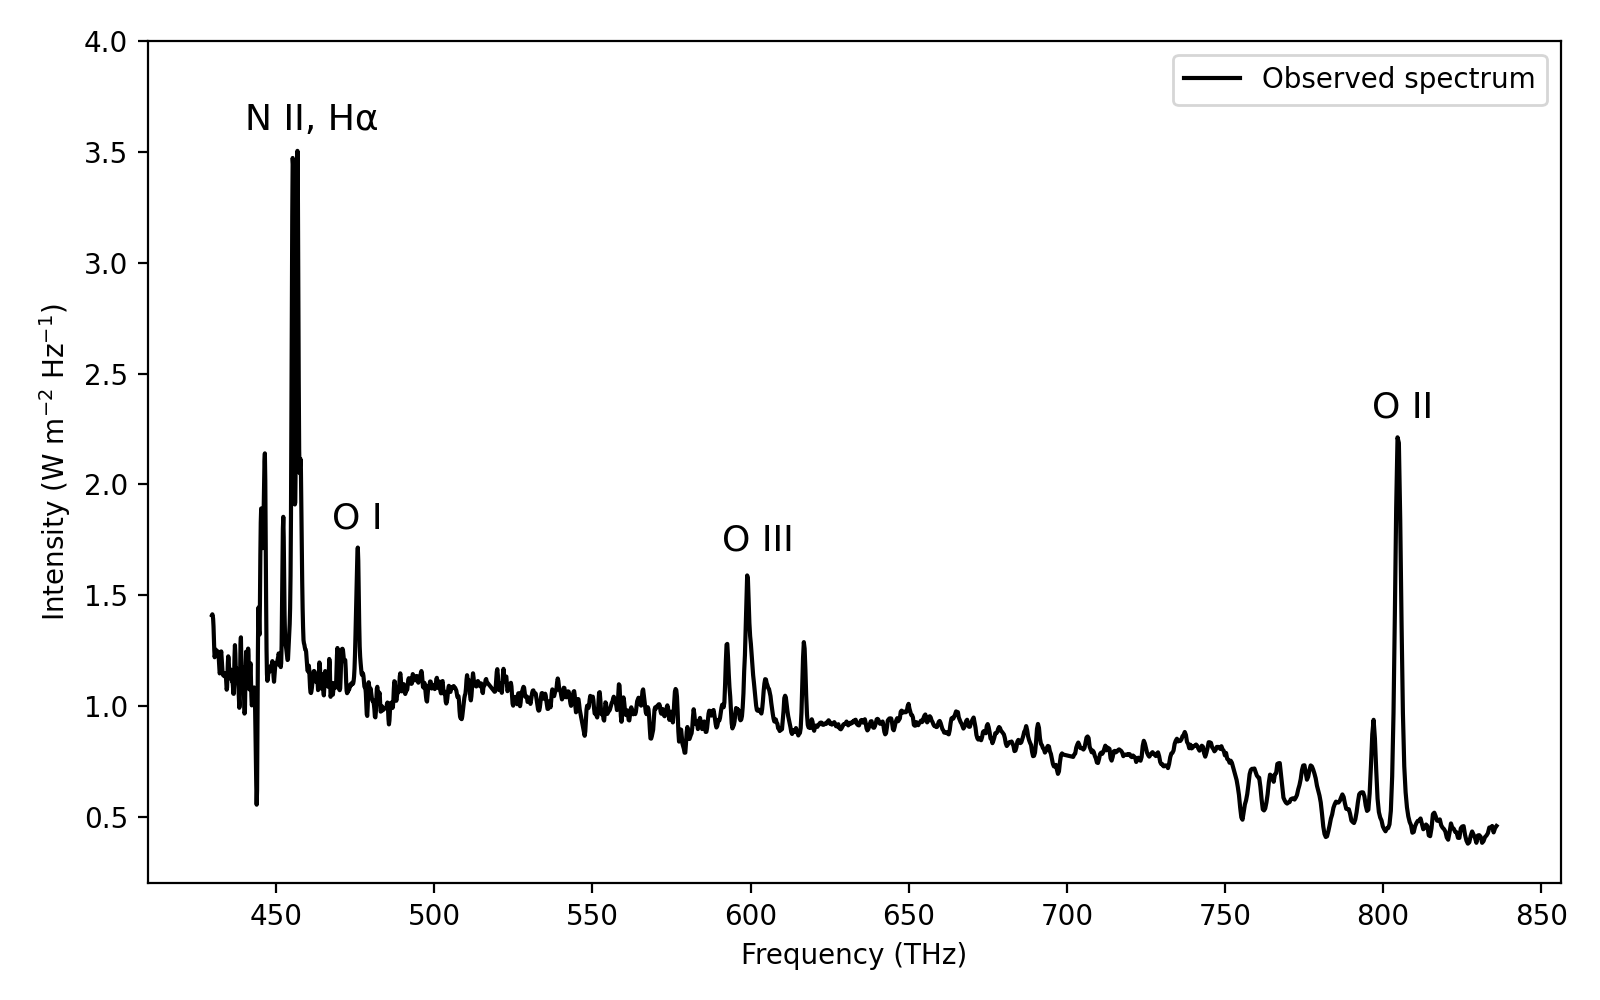
\includegraphics[width=0.7\linewidth]{Figures/3/final.png}
    \caption{Emission lines detected for galaxy NGC1275}
\label{galaxy_summary_pic}
\end{figure}

Note that by relaxing the threshold conditions, one can possibly find a few more low-strength emission lines. However, the accuracy will be low due to the high amount of noise in the spectrum.

Hence, we have successfully obtained line strengths and their corresponding chemical origin for for different spectral lines in the spectrum of galaxy NGC1275.